\mysubsectionformatted{Design Pattern Command}
\myparagraph{

    \begin{tcolorbox}[colback=blue!5!white, colframe=blue!75!black]
        Permette di trasformare una richiesta in un oggetto indipendente.
        \\In questo modo si possono:
        \begin{enumerate}
            \item scollegare il mittende di una richiesta dal destinatario.
            \item rendere le operazioni riutilizzabili.
            \item registrare e annullare operazioni.
            \item creare sequenze di comandi.
        \end{enumerate}
    \end{tcolorbox}
    \noindent\textit{Command} è ideale per implementare operazioni complesse e modulari
    che possono essere facilmente eseguite, annullate, memorizzate e organizzate in sequenza.

    \begin{center}
        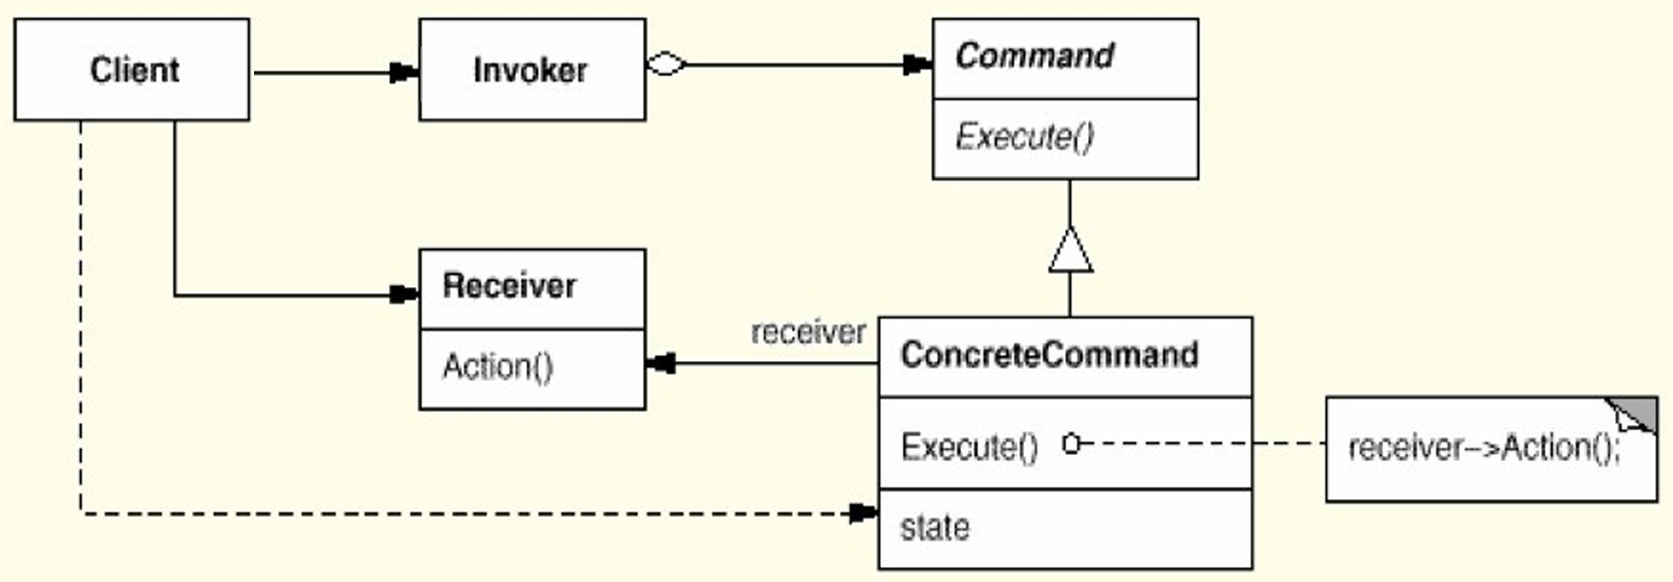
\includegraphics[scale=0.25]{Esercitazione - Design Patterns/command_pattern.png}
    \end{center}

    \begin{enumerate}
        \item \textbf{Client} è l'interfaccia che crea un'istanza concreta  \textbf{ConcreteCommmand}
              e ne imposta il \textbf{Receiver}.
        \item \textbf{\textit{Command}} è l'interfaccia per l'esecuzione dell'operazione.
        \item \textbf{ConcreteCommand} è la classe che incapsula l'operazione da eseguire
              in un oggetto specifico.
        \item \textbf{Invoker} è la classe che che richiede tramite il \textbf{\textit{Command}}
              l'esecuzione di una o più operazioni.
        \item \textbf{Receiver} è l'oggetto che esegue l'azione.
    \end{enumerate}

    \begin{center}
        \resizebox{\columnwidth}{!}{%
            \begin{tabular}{|l|}
                \hline
                \rowcolor[HTML]{32CB00}
                \multicolumn{1}{|c|}{\cellcolor[HTML]{32CB00}\textbf{Vantaggi}}                                                                                \\ \hline
                Separa l'oggetto che invoca l'operazione da quello che sa come eseguirlo                                                                       \\ \hline
                \begin{tabular}[c]{@{}l@{}}I \textit{Command} sono classi di oggetti e possono essere manipolati \\ come qualsiasi altro oggetto.\end{tabular} \\ \hline
                Si possono creare dei \textit{Command} composti.                                                                                               \\ \hline
                \'E semplice aggiungere nuovi \textit{Command}.                                                                                                \\ \hline
            \end{tabular}%
        }
    \end{center}
    \newpage
    \subsubsection{Esempio di Design Pattern Command}
    \begin{center}
        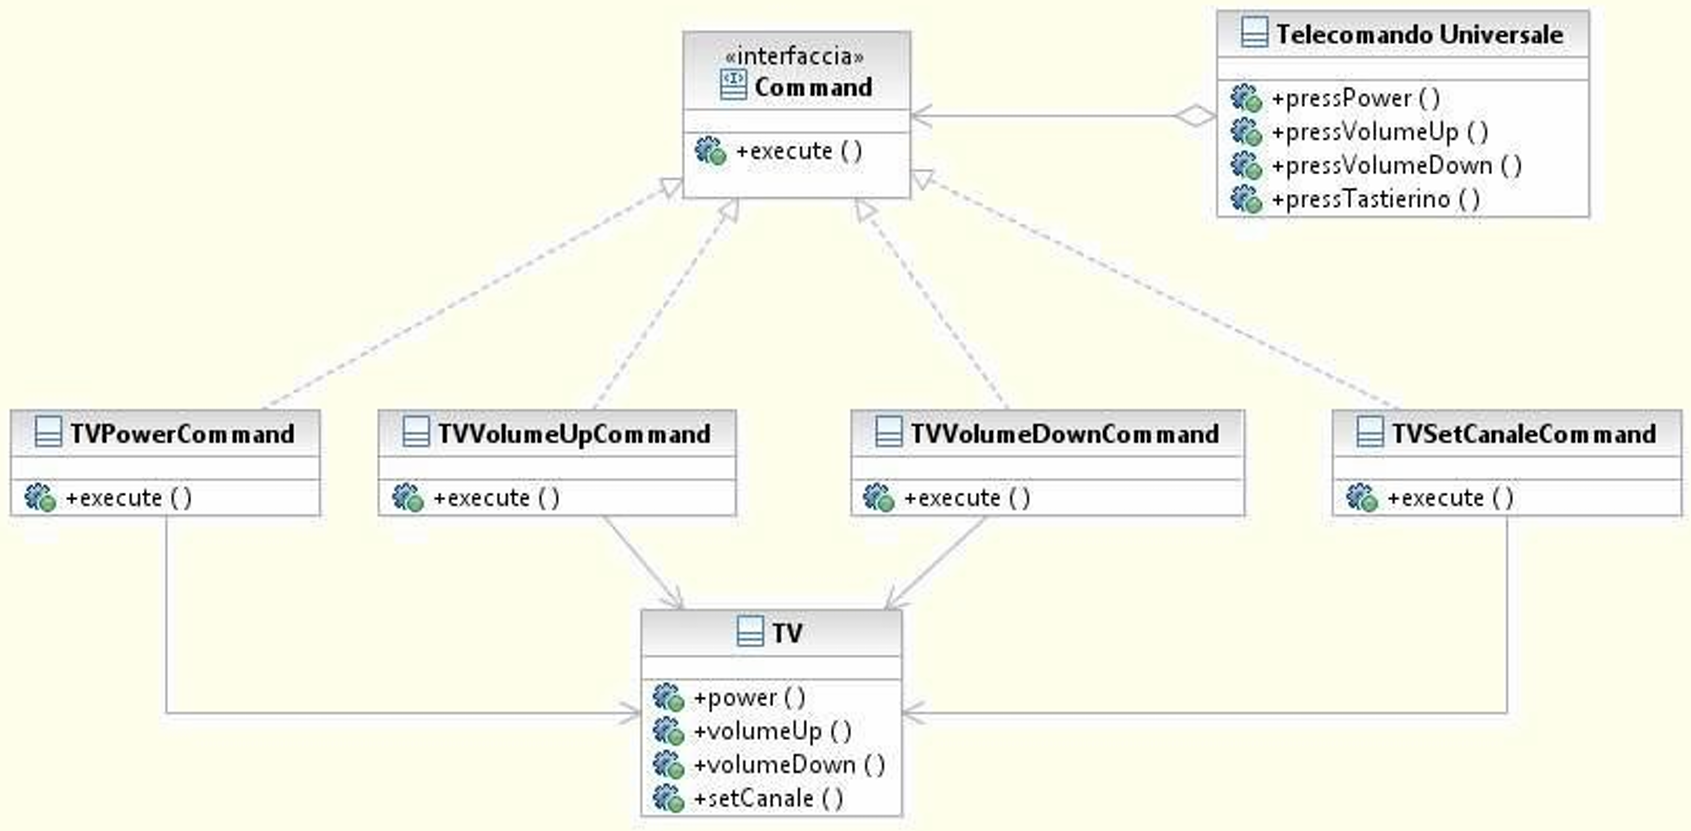
\includegraphics[scale=0.26]{Esercitazione - Design Patterns/example_command_pattern.png}
    \end{center}
    In questo esempio, \textbf{TV} è il \textbf{Receiver} che esegue l'azione stabilita dal \textbf{Telecomando Universale},
    ovvero l'\textbf{Invoker}. 
    \\
    I \textbf{ConcreteCommand} sono le 4 classi che ereditano il metodo \textbf{execute()} che
    invocano le corrispondenti operazioni del \textbf{Receiver}.
    \\
    Infine l'interfaccia \textbf{\textit{Command}} che definisce l'interfaccia alle classi concrete.
    \newpage

}